%\documentstyle[epsf,twocolumn]{jarticle}       %LaTeX2e仕様
\documentclass[twocolumn]{jarticle}     %pLaTeX2e仕様(platex.exeの場合)
% \documentclass[onecolumn]{ujarticle}   %pLaTeX2e仕様(uplatex.exeの場合)
%%%%%%%%%%%%%%%%%%%%%%%%%%%%%%%%%%%%%%%%%%%%%%%%%%%%%%%%%%%%%%
%%
%%  基本バージョン
%%
%%%%%%%%%%%%%%%%%%%%%%%%%%%%%%%%%%%%%%%%%%%%%%%%%%%%%%%%%%%%%%%%
\setlength{\topmargin}{-45pt}
%\setlength{\oddsidemargin}{0cm}
\setlength{\oddsidemargin}{-7.5mm}
%\setlength{\evensidemargin}{0cm}
\setlength{\textheight}{24.1cm}
%setlength{\textheight}{25cm}
\setlength{\textwidth}{17.4cm}
%\setlength{\textwidth}{172mm}
\setlength{\columnsep}{11mm}

%\kanjiskip=.07zw plus.5pt minus.5pt


% 【節が変わるごとに (1.1)(1.2) … (2.1)(2.2) と数式番号をつけるとき】
%\makeatletter
%\renewcommand{\theequation}{%
%\thesection.\arabic{equation}} %\@addtoreset{equation}{section}
%\makeatother

%\renewcommand{\arraystretch}{0.95} 行間の設定
%%%%%%%%%%%%%%%%%%%%%%%%%%%%%%%%%%%%%%%%%%%%%%%%%%%%%%%%
%\usepackage{graphicx}   %pLaTeX2e仕様(\documentstyle ->\documentclass)
\usepackage[dvipdfmx]{graphicx}
\usepackage{subcaption}
\usepackage{multirow}
\usepackage{amsmath}
\usepackage{url}
\usepackage{ulem}
\usepackage{algorithm}
\usepackage{algorithmic}
%%%%%%%%%%%%%%%%%%%%%%%%%%%%%%%%%%%%%%%%%%%%%%%%%%%%%%%%
\begin{document}

	%bibtex用の設定
	%\bibliographystyle{ujarticle}

	\twocolumn[
		\noindent
		\hspace{1em}
		2020 年 4 月 30 日
		ゼミ資料
		\hfill
		B4 杉山 竜弥
		\vspace{2mm}

		\hrule
		\begin{center}
			{\Large \bf 進捗報告}
		\end{center}
		\hrule
		\vspace{9mm}
	]

	% ‚ここから 文章 Start!
\section{今週やったこと}
	\begin{itemize}{ % itemize, enumerate, description
			\item{後述するデータを交換するアルゴリズムの実装と実験}
	}\end{itemize}

\section{問題設定}
% 何を入力として何を出力とするかを明確に定義

 データを正解と不正解に分割して学習する以下のアルゴリズム1を考える.

	\begin{algorithm}
		\caption{Swap two datasets}
		\label{alg1}
		\begin{enumerate}{ % itemize, enumerate, description
			\item{データ 2N 抜き出す}
			\item{そのデータを N(A) と N(B)に分ける.}
			\item{A → train, B → test で実験}
			\item{B → train, A → test で実験}
			\item{3.と4.で test でミスしたデータを調べる}
			\item{A をテストとしたとき失敗したデータと B をテストとしたとき成功したデータを入れ替える.}
			\item{3.に戻る.}
		}\end{enumerate}
			% \begin{algorithmic}
			% \end{algorithmic}
	\end{algorithm}

	アルゴリズム1の手順6の操作によって, データセットAには成功データ, Bには失敗データが集められる.
	従って簡単なデータを学習し, 難しいデータでテストされる手順3の精度は低くなると予想される.

	アルゴリズム1に示した手順の設定として, 手順 3. 4.で2つのモデルをそれぞれ独立させた. またデータポイントの入れ替えは, 入れ替え可能なデータを先頭から全て交換することにした.

\section{実験}
% \section{現在の状況}
% 何を使ってどのくらいの精度が出ているか?

\begin{description}{ % itemize, enumerate, description
		\item[実験1]{アルゴリズム1で学習}
		\item[実験2]{データ交換の実装をテストするため, 手順 3. 4.で訓練を行わずアルゴリズム1を学習}
		\item[実験3]{ベースラインとしてデータ数をNのまま, データを入れ替えず学習}
}\end{description}

\subsection{共通実験設定}

	実験 1 ~ 3 は, 条件にない限り表\ref{tab:setting}の設定に従って学習した. データセットに CIFAR10\cite{CIFAR10}を利用したため, モデルに与える問題は10クラス識別とした. 入力は 3 channel x 32 pix x 32 pixの画像で, 出力は 10クラスの確率である. 多クラス識別のため損失関数は Cross Entropy Lossを利用した.
	手順 3. 4.の実験の期間は, 1 epochと設定して, 25 epochで25 回の入れ替えを行った.

	\begin{table}[tb]
	  \begin{center}
	    \caption{実験の設定}
	    \begin{tabular}{|c|c|} \hline
				dataset & cifar10 \\
				data N & 25,000 / model \\ \hline
	      task & 10クラス識別 \\
	      input & image(3x32x32) \\
				output & class(10) \\ \hline
	      model & CNN \\
	      optim & SDG (lr=0.001, moment=0.9) \\
	      loss & Cross Entropy Loss \\ \hline
	      batch size & 16 \\
	      epoch & 25 \\ \hline
	    \end{tabular}
	    \label{tab:setting}
	  \end{center}
	\end{table}

\subsection{実験結果}

\begin{table}[tb]
	\begin{center}
		\caption{実験2の手順6の結果}
		\begin{tabular}{|c|c|c|} \hline
			テスト & 結果(o:正解, x:不正解) & 交換 \\ \hline
			A & x x x x x x x o x o & 1番目 \\
			B & x x o x x x x x x x & 3番目 \\ \hline
		\end{tabular}
		\label{tab:swap}
	\end{center}
\end{table}

\subsubsection{実装の確認}
 実験2での入れ替え例を表\ref{tab:swap}に示した. 一部抜き出した10件のデータで, 先頭から期待通りに交換されていることを確認した. また全体として, 図\ref{fig:accuracy}のテストの精度から, 1 epoch目でほとんどのデータが交換されたことが分かる. 以上より実装に問題がないと判断した.
	% 損失の変化を図\ref{fig:loss}, テストの精度を図\ref{fig:accuracy}に示した.
%  まず実験2の結果から実装を確認すると, 図\ref{fig:accuracy}よりデータセットBから正解したデータがほとんど交換されたことが分かる. 一方学習していないため, Bで偶然正解したデータはAで不正解となりデータセットBの精度はほぼ変化していない.

\subsubsection{実験1の結果と考察}
	図\ref{fig:accuracy}のように予想通り手順3は学習を重ねるごとに, 精度が下がり0.992 [\%]になった. 反対に手順4は学習が進み, 精度は38.3 [\%]となった. 一方で実験3の通常の学習では同数のデータセットかつ同一条件で, 最も高い56.0 [\%]となった. 実験3と比較して20 [\%]程度精度が劣った理由は, データセットが頻繁に操作され不安定であることや, データの多様性が失われたことによる汎化能力の低下が考えられる.

	図\ref{fig:accuracy}の手順4のグラフで精度が交互に激しく変化する現象が見られた. これデータセットが入れ替えによって, 難易度が大きく変化しテストに影響していると思われる. しかしデータの流れやテストの難易度は分かっていないため, 調査が必要である.


	% \begin{figure}[tbhp]
	% 	\begin{center}
	% 		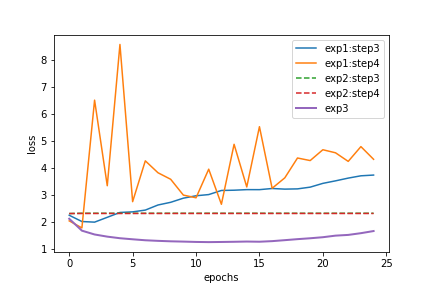
\includegraphics[clip,width=8.5cm]{loss.png}
	% 		\caption{損失の推移 
	% 		(実験1)実線の青が手順3, 橙が手順4, 不安定で増加傾向.
	% 		(実験2)点線の緑と赤, 変化しない.
	% 		(実験3)太線の紫, 減少しているが後半微増.}
	% 		\label{fig:loss}
	% 	\end{center}
	% \end{figure}

	\begin{figure}[tb]
		\begin{center}
			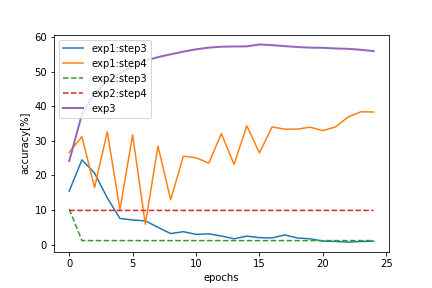
\includegraphics[clip,width=8.5cm]{accuracy.png}
			\caption{テストの精度 
			(実験1)実線の青が手順3で0に近い精度, 橙が手順4で不安定に向上.
			(実験2)点線の緑が手順3, 赤が手順4でベースラインに近い.
			(実験3)太線の紫, 最も高い精度.}
			\label{fig:accuracy}
		\end{center}
	\end{figure}

% \subsection{考察}

% \section{前回からの進捗}
% あれば報告

\section{現在の問題点}
% 精度が出ない,とかだけではなく自分なりの考察を示す
現在の実装では, 入れ替えを先頭から全て行うように設定している. 偏りをなくすためランダムに選択したり, 一部のみを入れ替えられる必要がある.

ベースラインのCNNの精度が高くなかったため, CNNを改良し結果を比較したい.

精度の変化を説明するため, 入れ替えたデータの量を測りデータの流れを分析したい.

入れ替える実験の期間として, 1 epochが適切かどうかが不明のため, 最適な期間を探す実験が必要な可能性がある.

実装について, CPUで行っているデータの入れ替えをGPUで再実装し, 高速化したい.

\section{現在のソースコード}
% 埋め込みでもGitでもいいので参照できるように
モデルの実装はGithub
\footnote[1]{\url{https://github.com/tatsuya-sugiyama/WeeklyReport/blob/master/test/AB_split.ipynb}}
を参照.


\section{今後の予定}
% なんとなくなんかの勉強をするとかではなく具体的に

\begin{itemize}{ % itemize, enumerate, description
		\item{具体的なデータを分析し, 精度の妥当性について考察する}
		\item{Pytorchを調べて, GPUによる演算を実装し, 学習時間の短縮を行う}
}\end{itemize}

	% \begin{figure}[htbp]
	% 	\begin{center}
	% 		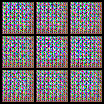
\includegraphics[clip,width=7.0cm]{../../test/images/0.png}
	    % 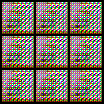
\includegraphics[clip,width=7.0cm]{../../test/images/3100.png}
	% 		\caption{学習結果 左:0 epoch, 右:1 epoch (32x32)}
	% 		\label{fig:result}
	% 	\end{center}
	% \end{figure}

	% 参考文献リスト
	\bibliographystyle{unsrt}
	\bibliography{ref}
\end{document}
